% 饱和蒸汽压
% 水蒸气|汽压|理想气体

\pentry{理想气体分压定律\upref{PartiP}}

在一定的温度下, 若容器中某种液体和它的蒸汽达到平衡, 这是气体的压强就是\textbf{饱和蒸汽压}. 注意饱和蒸汽压只和液体的种类和温度有关.

我们用一个函数 $P_\alpha(T)$ 描述饱和蒸汽压和温度的关系. 例如水蒸气的饱和蒸汽压记为 $P_{H2O}(T)$ (\autoref{VaporP_fig2}). 若容器的体积可以变化, 当容器变大而温度不变时, 压强首先会变小, 但液体会继续汽化, 直到压强恢复到饱和蒸汽压时重新达到平衡. 反之, 当容器体积变小(温度不变), 则压强首先升高,  然后气体会逐渐液化直到恢复饱和蒸汽压时重新达到平衡. 一般来说, 温度升高会导致饱和蒸汽压升高.

为了方便讨论, 我们以下假设蒸汽为理想气体. 在常温常压(或更低温低压)下这一般是近似成立的, 但在高温高压下假设会失效.

\begin{figure}\label{VaporP_fig2}[ht]
\centering
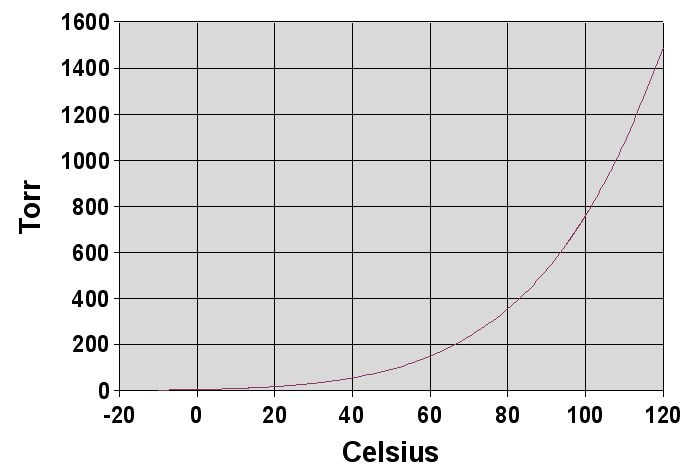
\includegraphics[width=10cm]{./figures/VaporP1.png}
\caption{水的饱和蒸汽压, 横坐标是摄氏温度, 纵坐标是毫米汞柱(图片来自维基百科)} \label{VaporP_fig1}
\end{figure}

\begin{exercise}{水蒸气的质量}
根据\autoref{VaporP_fig2} 和理想气体状态方程, 求 25° 时一立方米纯水蒸气的质量.
% 未完成
\end{exercise}

\subsection{混合气体}
我们接下来讨论容器中除了某种液体及其蒸汽外, 还有另一种气体的情况. 例如水, 水蒸气和干燥的空气. 如果将两种气体都视为理想气体, 那么两种气体的总压强可以根据分压定律来计算, 即水蒸气单独存在时的压强加上空气单独存在时的压强. 另外, 假设空气分子不溶于水且不与水分子发生任何反应, 则水蒸气的分压仍然是 $P_{H2O}(T)$.

令干燥空气的分压为 $P_{air}$ 则混合气体总压强 $P$ 为
\begin{equation}
P = P_{H2O}(T) + P_{air}
\end{equation}
所以若已知总压强和温度, 平衡时两种气体的比例为
\begin{equation}\label{VaporP_eq1}
\frac{n_{H20}}{n_{air}} = \frac{P_{H2O}(T)}{P_{air}} = \frac{P_{H2O}(T)}{P - P_{H2O}(T)}
\end{equation}
注意该式中温度必须低于某个值, 使分母大于零. 下面我们会看到, 这个值就是压强 $P$ 下的沸点.

\subsection{相对湿度绝对湿度}
我们下面来介绍日常生活中经常使用的相对湿度. 我们先定义\textbf{绝对湿度}为 $n'_{H20}/n'_{air}$, 这里使用一瞥表示实际上的比例而不是平衡时的比例(\autoref{VaporP_eq1}). 若 $P$ 表示大气压强, 那么\autoref{VaporP_eq1} 就是某温度和汽压下可能出现的\textbf{最大绝对湿度}. 因为如果实际湿度稍高于这个值, 空气中的水蒸气就会迅速凝结到空气中的尘埃上, 形成云或雾, 有或者直接凝结到物体表面形成水滴或霜.

另一方面, 空气中绝对湿度常常低于\autoref{VaporP_eq1} 的值, 即水和水蒸气处于不平衡的状态. 这是因为地表的水(江湖海, 湿润的土壤等)蒸发的速度有限.

我们把\textbf{相对湿度}定义为当前的绝对湿度除以当前温度和压强的最大绝对湿度, 即
\begin{equation}
\left. \frac{n'_{H20}}{n'_{air}} \middle/ \frac{n_{H20}}{n_{air}} \right.
\end{equation}

\subsection{沸腾}

(未完成)
